\documentclass[english, DIV=13]{scrartcl}

% Packages
\usepackage[utf8x]{inputenc}
\usepackage[T1]{fontenc}
\usepackage{lmodern}
\usepackage{microtype}
\usepackage{xspace}
\usepackage[binary-units=true]{siunitx}
\usepackage{graphicx}
\usepackage{hyperref}
\usepackage{todonotes}
\usepackage{epstopdf}
\usepackage{array}
\usepackage{multicol}
\usepackage{multirow}
\usepackage{tabularx} % tabular with automatic line-break
\newcolumntype{Y}{>{\centering\arraybackslash}X} % centered column
\usepackage{amsmath}
\usepackage{grffile} % better name handling with graphicx
\usepackage{currfile} % provides relative file inclusion for tikzscale
\usepackage{placeins}

\usepackage{caption}
\usepackage{subcaption}

\usepackage{tikz}
\usepackage{pgfplots}
\usepackage{pgfplots}
\usepackage{tikzscale}
\pgfplotsset{compat=newest}
\usetikzlibrary{plotmarks}
\usepackage{rotating}
\usepackage[absolute,overlay]{textpos}
\usepackage{circuitikz}

% Math symbols
\usepackage{amsmath}
\usepackage{amssymb}
\usepackage{amsthm}
\DeclareMathOperator*{\argmin}{arg\,min}
\DeclareMathOperator*{\argmax}{arg\,max}
\newcommand\norm[1]{\left\lVert#1\right\rVert}
\DeclareMathOperator{\erfc}{erfc}

% Sets
\newcommand{\Z}{\mathbb{Z}}
\newcommand{\R}{\mathbb{R}}
\newcommand{\Rn}{\R^n}
\newcommand{\Rnn}{\R^{n \times n}}
\newcommand{\C}{\mathbb{C}}
\newcommand{\K}{\mathbb{K}}
\newcommand{\Kn}{\K^n}
\newcommand{\Knn}{\K^{n \times n}}

% Unit vectors
\usepackage{esint}
\usepackage{esvect}
\newcommand{\kmath}{k}
\newcommand{\xunit}{\hat{\imath}}
\newcommand{\yunit}{\hat{\jmath}}
\newcommand{\zunit}{\hat{\kmath}}
\newcommand{\uunit}{\hat{\umath}}

% rot & div & grad & lap
\DeclareMathOperator{\newdiv}{div}
\newcommand{\divn}[1]{\nabla \cdot #1}
\newcommand{\rotn}[1]{\nabla \times #1}
\newcommand{\grad}[1]{\nabla #1}
\newcommand{\gradn}[1]{\nabla #1}
\newcommand{\lap}[1]{\nabla^2 #1}

% Elec
\newcommand{\B}{\vec B}
\newcommand{\E}{\vec E}
\newcommand{\EMF}{\mathcal{E}}
\newcommand{\perm}{\varepsilon} % permittivity

\newcommand{\bigoh}{\mathcal{O}}
\newcommand\eqdef{\triangleq}

\DeclareMathOperator{\newdiff}{d} % use \dif instead
\newcommand{\dif}{\newdiff\!}
\newcommand{\fpart}[2]{\frac{\partial #1}{\partial #2}}
\newcommand{\ffpart}[2]{\frac{\partial^2 #1}{\partial #2^2}}
\newcommand{\fdpart}[3]{\frac{\partial^2 #1}{\partial #2\partial #3}}
\newcommand{\fdif}[2]{\frac{\dif #1}{\dif #2}}
\newcommand{\ffdif}[2]{\frac{\dif^2 #1}{\dif #2^2}}
\newcommand{\constant}{\ensuremath{\mathrm{cst}}}

\usepackage[margin=0.5in]{geometry}
\usepackage{placeins}
\usepackage{pgfplots}
\usepackage{amsmath,amsfonts,amssymb}
\usepackage{empheq}
\usepackage{hyperref}
\usepackage{todonotes}
\newcommand\norm[1]{\left\lVert#1\right\rVert}
\renewcommand{\vec}[1]{\mathbf{#1}}

\title{LINMA1731 - Project}
\author{Antoine Paris\and Matthieu Xhonneux}
\date{\today}

\begin{document}
\maketitle

\section{Discrete-time version of the Lorenz system}
Using first-order forward finite difference, the Lorenz dynamical system can be written as
\[ \vec{x}_{k+1} = F(\vec{x}_k) + \Gamma\vec{u}_k \]
where the function $F$ is given by
\begin{equation*}
    \begin{cases}
        F_1(\vec{x}_k) &= ay_k\delta t + (1-a\delta t)x_k \\
        F_2(\vec{x}_k) &= x_k(r-z_k)\delta t + (1-\delta t)y_k \\
        F_3(\vec{x}_k) &= x_ky_k\delta t + (1-b\delta t)z_k
    \end{cases}.
\end{equation*}

\section{Discrete-time system simulation and observation}
A sample trajectory resulting from a 50 seconds simulation is given in figure~
\ref{fig:q2-3d-trajectory}. As expected for this set of paramaters, the trajectory
is chaotic and shows the typical ``figure eigth'' form. 
The trajectory of the first coordinates and the corresponding noisy measurements
with $\sigma^2_m = 1$ are represented in figure~\ref{fig:q2-mes-vs-real}.
\begin{figure}[hb]
    \centering
    \begin{subfigure}{0.49\textwidth}
        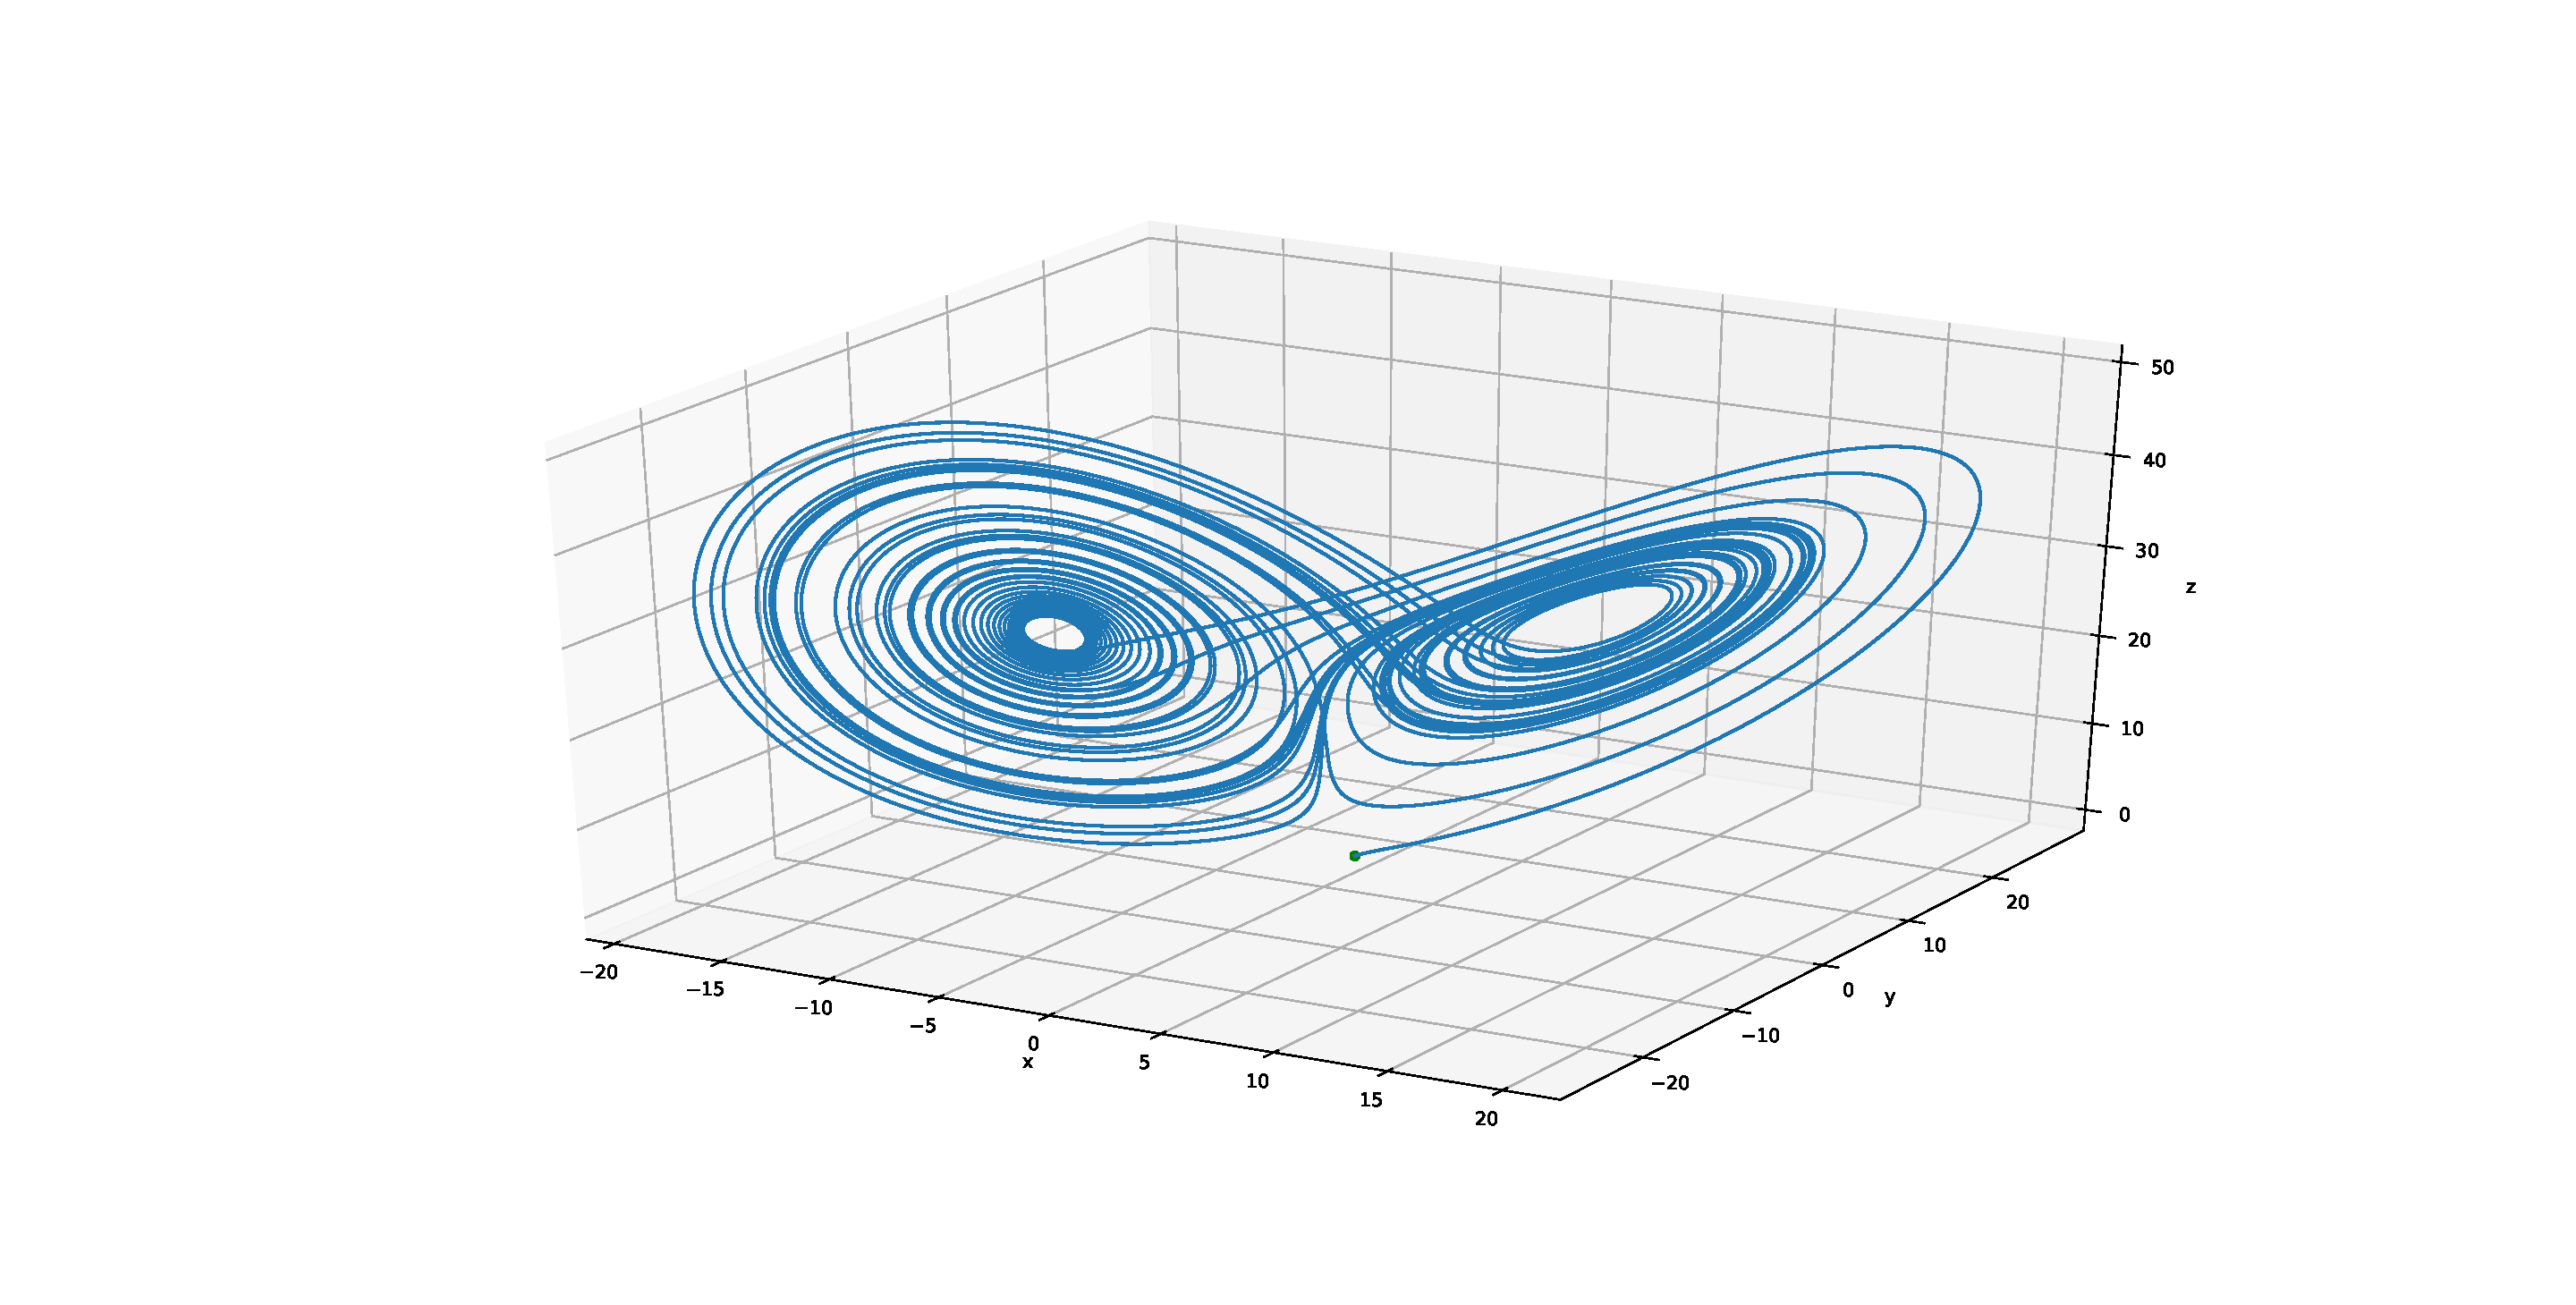
\includegraphics[width=\textwidth]{figures/q2-3d-trajectory}
        \caption{Realization of a 50 seconds simulated trajectory. The initial
        position is indicated by the green dot.}
        \label{fig:q2-3d-trajectory}
    \end{subfigure}%
    ~
    \begin{subfigure}{0.49\textwidth}
        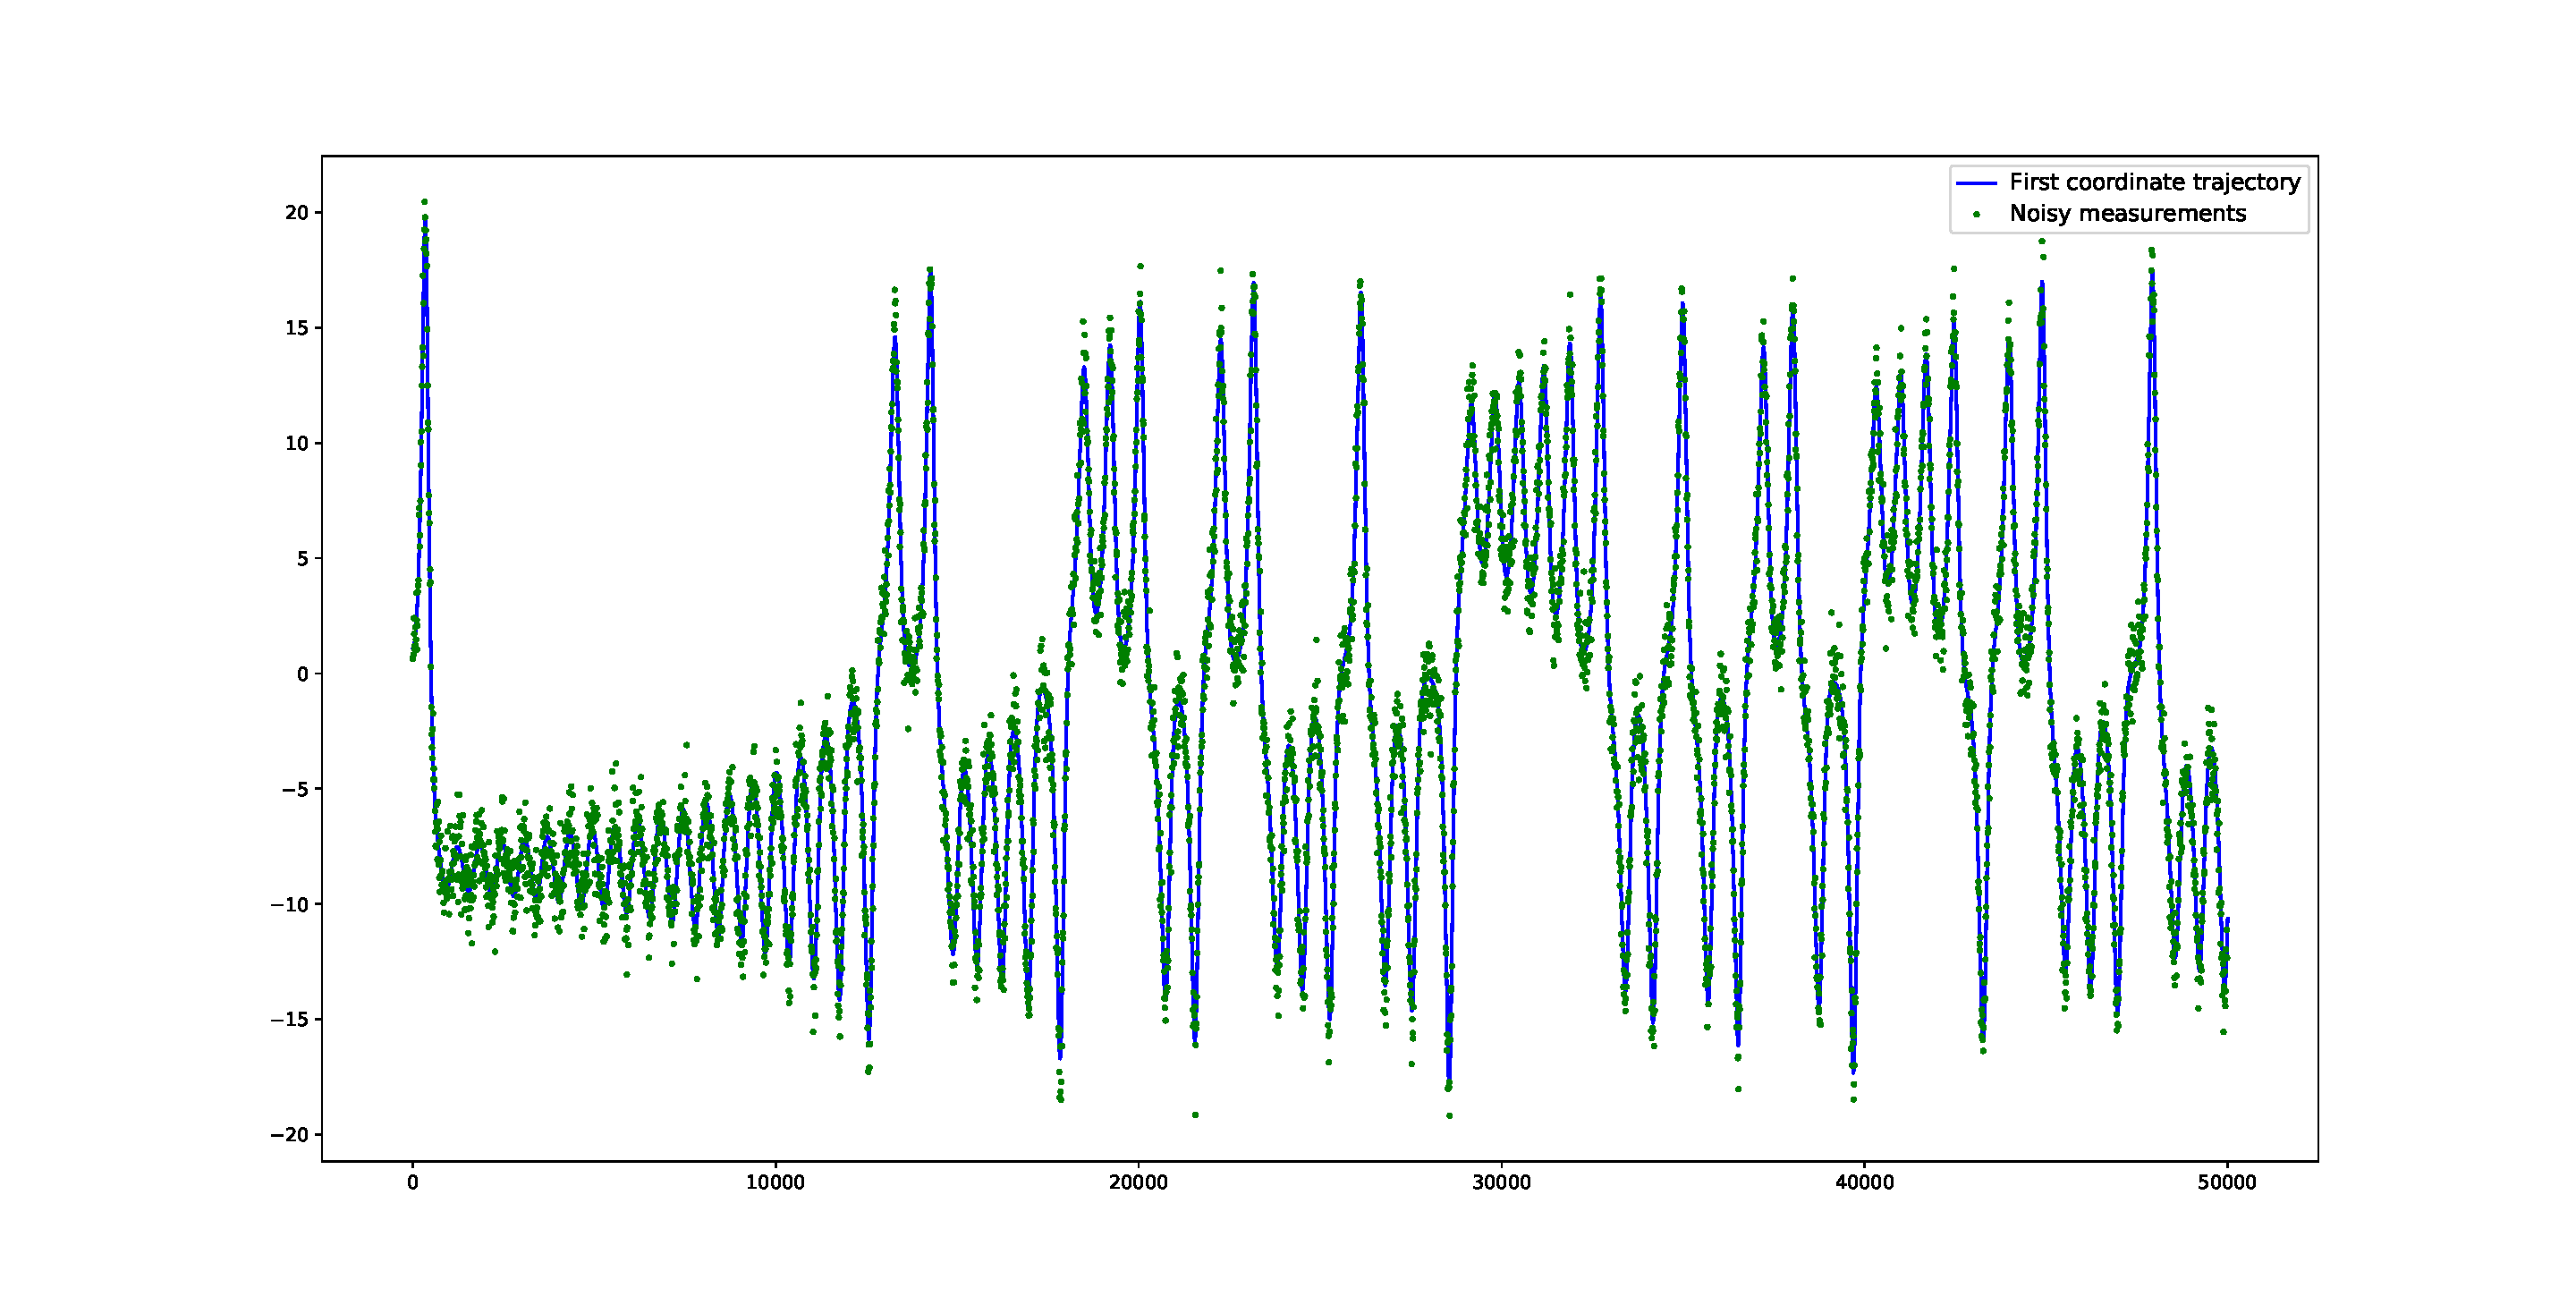
\includegraphics[width=\textwidth]{figures/q2-mes-vs-real}
        \caption{Trajectory of the first coordinates and corresponding noisy
        measurements with $\sigma^2_m = 1$.}
        \label{fig:q2-mes-vs-real}
    \end{subfigure}
    \caption{Simulations and measurements.}
\end{figure}

\FloatBarrier

\section{Sequential Monte Carlo}
\subsection{Particles distribution}
Histograms of the samples distribution in $x_k$ and $y_t$ for $t = 5, 10, 15$ are
given in figures~\ref{fig:q3-hist-x-100} and \ref{fig:q3-hist-y-100} respectively
(after resampling). These two figures shows that the particles tend to be normally
distributed around the real value. This is even more true when the number of particles
increases (with 1000 particles for example).

\begin{figure}
    \centering
    \begin{subfigure}{0.49\textwidth}
        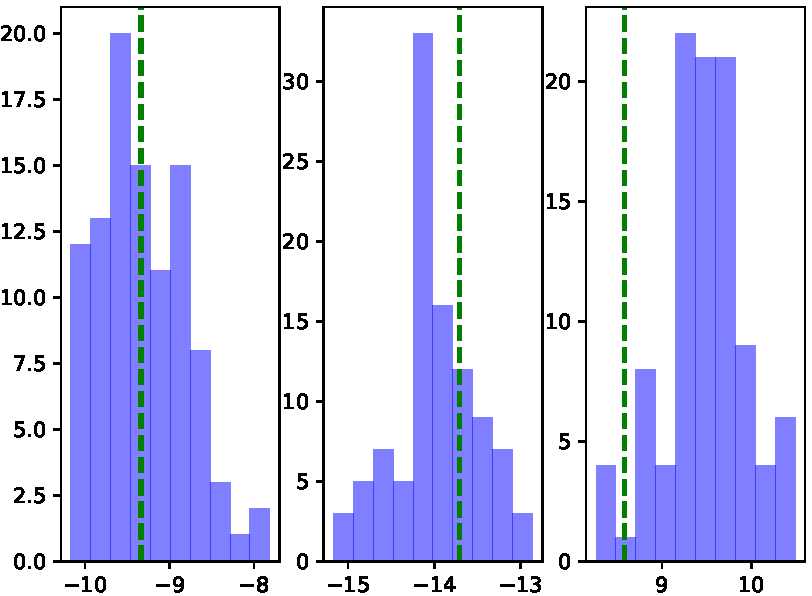
\includegraphics[width=\textwidth]{figures/hist-x-100}
        \caption{Histogram of samples distributions in $x_k$.}
        \label{fig:q3-hist-x-100}
    \end{subfigure}%
    ~
    \begin{subfigure}{0.49\textwidth}
        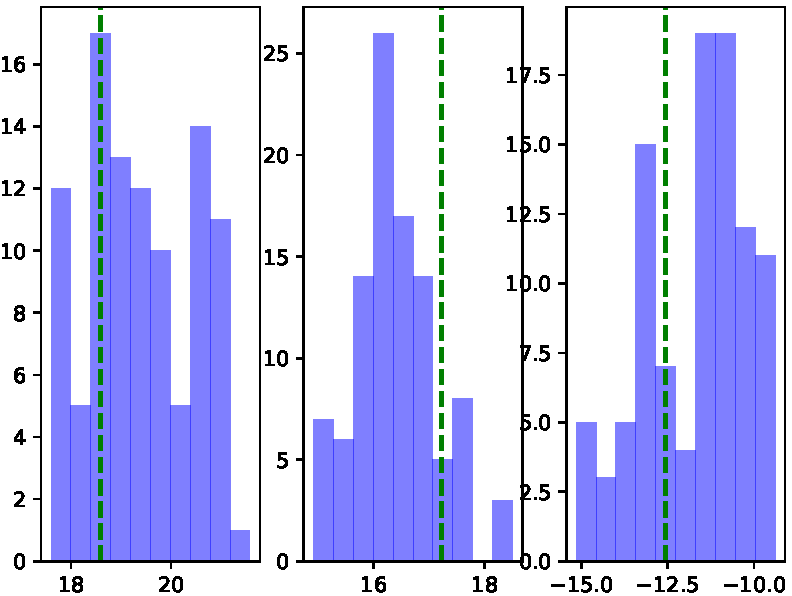
\includegraphics[width=\textwidth]{figures/hist-y-100}
        \caption{Histogram of samples distributions in $y_k$.}
        \label{fig:q3-hist-y-100}
    \end{subfigure}
    \caption{Histogram of samples distributions  at time $t = 0, 5, 15$
    (from left to right) for 100 particles. The dashed green lines represent the real
    values.}
    \label{fig:q3-hist}
\end{figure}

\subsection{Particles resampling}
Particles importance resampling is illustrated in figures~\ref{fig:particle-5-100}
and~\ref{fig:particle-15-100} for 100 particles. The ojective of this importance
resampling is to choose the most probables particles with respect to the observed
value. One can visually check from the histograms of the preceding section (which
contains the real value as a dashed green line) that the resampled particles indeed tend
to concentrate around the real value.

\begin{figure}
    \centering
    \begin{subfigure}{0.49\textwidth}
        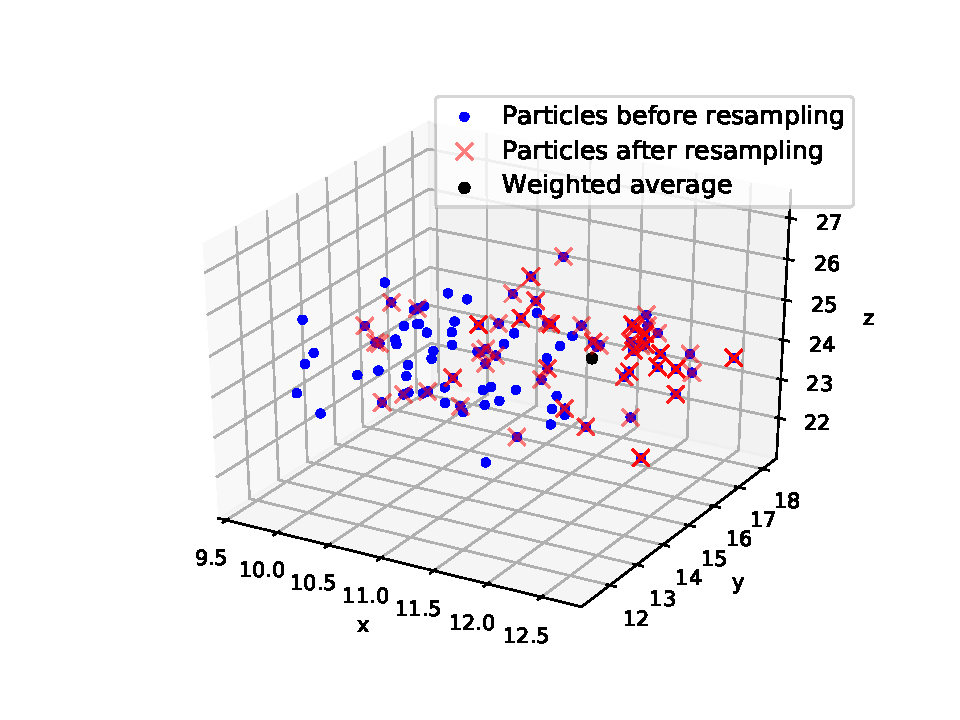
\includegraphics[width=\textwidth]{figures/particles-5-100}
        \caption{At $t=5$.}
        \label{fig:particle-5-100}
    \end{subfigure}%
    ~
    \begin{subfigure}{0.49\textwidth}
        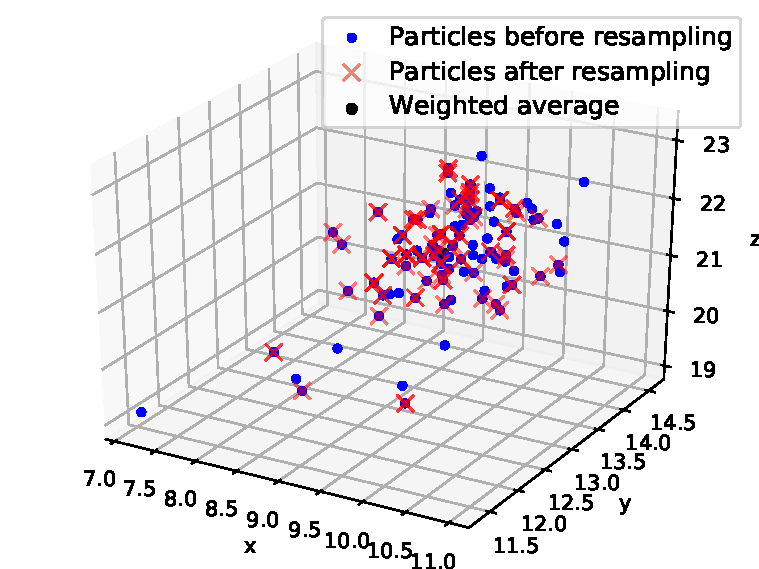
\includegraphics[width=\textwidth]{figures/particles-15-100}
        \caption{At $t=15$.}
        \label{fig:particle-15-100}
    \end{subfigure}
    \caption{Particles before and after resampling for 100 particles.
    Transparence level of red crosses indicates if particles have been chosen
    multiples times (the less transparent, the more a particle has been chosen).}
\end{figure}

\subsection{Estimation error}
Estimation errors, measured as 
$\norm{\mathbf{x}_t^{\text{real}} - \sum_{i=1}^n w_t^i\tilde{\mathbf{x}}_t^i}_2$,
are given in figure~\ref{fig:q3-error-50}, \ref{fig:q3-error-100} and
\ref{fig:q3-error-1000} for $n = 50, 100, 1000$ particles repectively.
From these figures, it can be observed that the estimation error decreases with the
number of particles. This is linked to the observations made previously about the
particles distribution. The higher the number of particles, the more this distribution
is close to a normal centered on the real value. Peak of large errors also seems to
rarify with higher number of particles. This can be explained as follows: an higher
number of particles means a larger diversity across the particles and a larger diversity
means a better ability to cope with large fluctuations in the dynamics of the system.

\begin{figure}
    \centering
    \begin{subfigure}{0.49\textwidth}
        \centering
        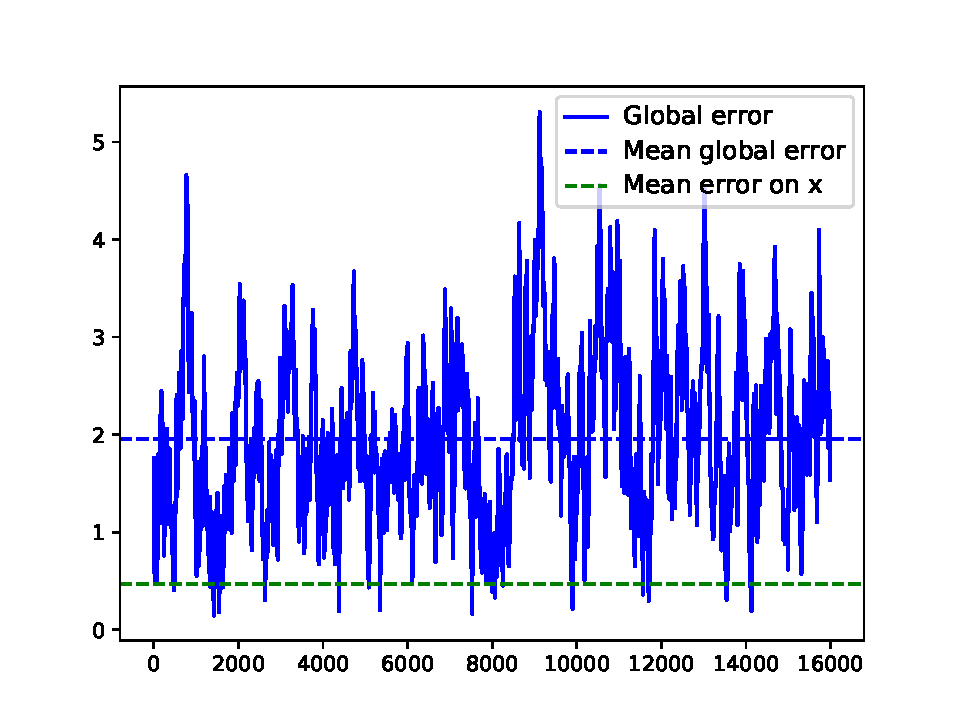
\includegraphics[width=0.9\textwidth]{figures/error-50}
        \caption{For $n=50$ particles.} 
        \label{fig:q3-error-50}
    \end{subfigure}%
    ~
    \begin{subfigure}{0.49\textwidth}
        \centering
        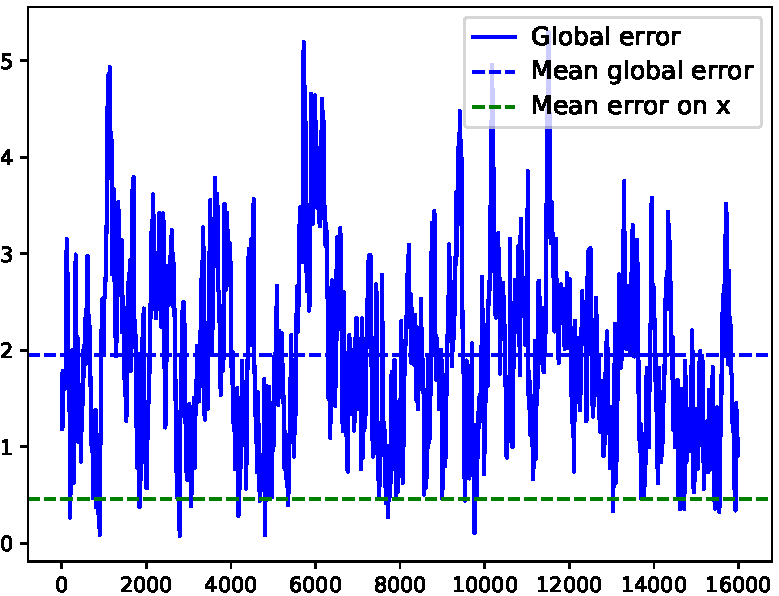
\includegraphics[width=0.9\textwidth]{figures/error-100}
        \caption{For $n=100$ particles.} 
        \label{fig:q3-error-100}
    \end{subfigure}\\
    \begin{subfigure}{0.49\textwidth}
        \centering
        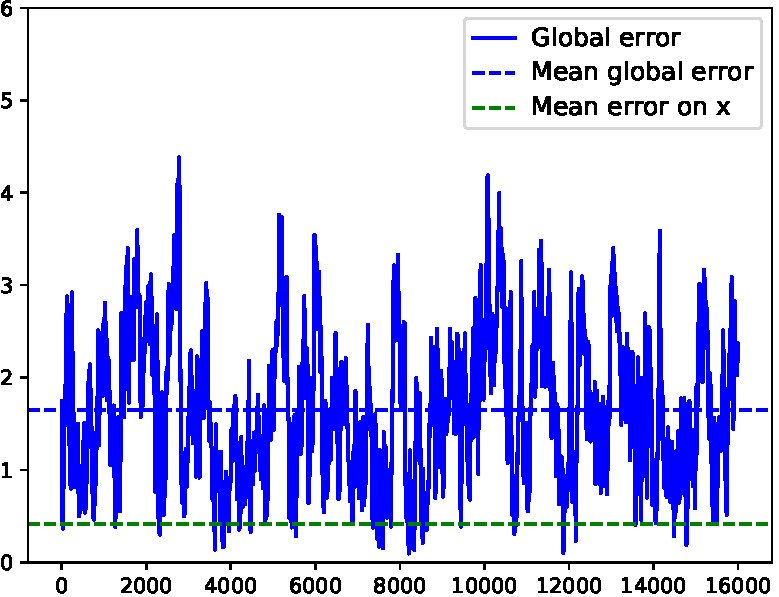
\includegraphics[width=0.9\textwidth]{figures/error-1000}
        \caption{For $n=1000$ particles.} 
        \label{fig:q3-error-1000}
    \end{subfigure}
    \caption{Error as a function of time for different numbers of particles. The blue
    lines correspond toi
    $\norm{\mathbf{x}_t^{\text{real}} - \sum_{i=1}^n w_t^i\tilde{\mathbf{x}}_t^i}_2$.
    The mean error on the first coordinate has also been plotted.}
\end{figure}

\subsection{Experiments}
\paragraph{Effect of $\sigma^2_u$}
The noise on the dynamics $\sigma^2_u$ highly impacts the diversity of the particles set.
A too small $\sigma^2_u$ causes the particles set to quickly degenerate, that is to
contain only a few number of very close particles. When this happens, the algorithm is
no longer able to efficiently estimate the trajectory and the error skyrockets. Larger
value of $\sigma^2_u$ adds uncertainty on the dynamics of the system. This obviously
limits the accuracy of the prediction made by the algorithm but helps a lot to keep
a diverse set of particles.

\paragraph{Effect of $\sigma^2_0$}
The variance of the initial position $\sigma^2_0$ can be seen as how much
\textit{a priori} knowledge on the initial position the algorithm has.
Intuitively, if $\sigma^2_0$ is large, the algorithm will generate a diverse initial set
of particles. If $\sigma^2_0$ is small, the algorithm will generate an initial set more
concentrated on the mean initial position. As a consequence, a large $\sigma^2_0$ might
lead to a large initial estimation error before the particle set concentrates more. This
was indeed observed on a simulation with 100 particles and a very large $\sigma^2_0$ where
peak errors up to a value of 10 appear initialy. However, the situation then quickly goes
back the normal. This is illustrated in figure~\ref{fig:error-100-s0-high}.

\begin{figure}
    \centering
    \begin{subfigure}{0.49\textwidth}
        \centering
        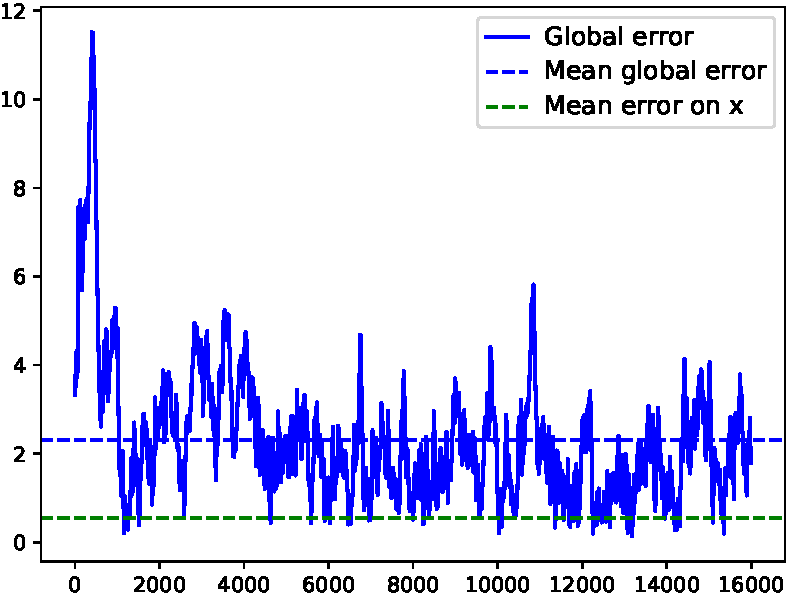
\includegraphics[width=0.8\textwidth]{figures/error-100-s0-high}
        \caption{Effect of a large $\sigma^2_0$.}
        \label{fig:error-100-s0-high}
    \end{subfigure}%
    ~
    \begin{subfigure}{0.49\textwidth}
        \centering
        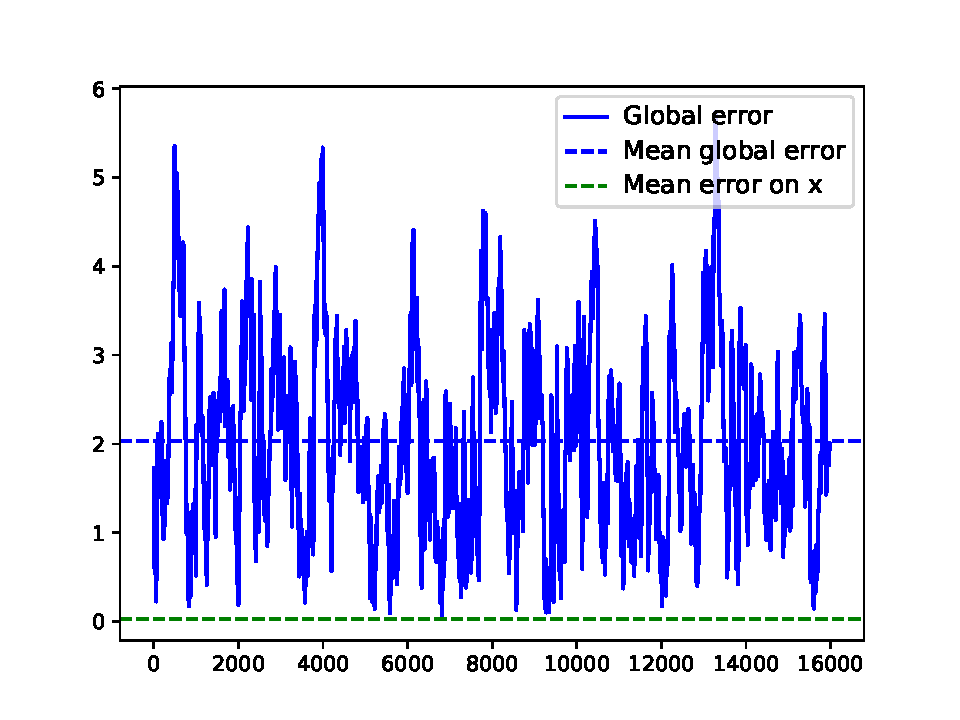
\includegraphics[width=0.8\textwidth]{figures/error-100-sm-low}
        \caption{Effect of a small $\sigma^2_m$.}
        \label{fig:error-100-sm-low}
    \end{subfigure}
    \caption{Effect of $\sigma^2_0$ and $\sigma^2_m$ on the error on SMSC with
    100 particles.}
\end{figure}

\paragraph{Effect of $\sigma^2_m$}
The variance of the measurement noise $\sigma^2_m$ mainly impacts the estimation error on
the first coordinate. Figure~\ref{fig:error-100-sm-low} shows the error curve for a very
low $\sigma^2_m$. The mean error on the first coordinate (dashed green line) is indeed
a lot smaller than in figure~\ref{fig:q3-error-1000} where $\sigma^2_m = 1$ for example.
On the other hand, the global error (i.e. $\norm{\mathbf{x}_t^{\text{real}} -
\sum_{i=1}^n w_t^i\tilde{\mathbf{x}}_t^i}_2$) does not vary much with $\sigma^2_m$.
Indeed, even if the mean error on $x$ decreases, the errors on $y$ and $z$ will not
necessarily decrease.

\paragraph{Effect of $\delta t$ and $\Delta t$}
The effect of the ratio of $\Delta t$ to $\delta t$ will now be discussed. Intuitively,
having $\Delta t/\delta t = 1$ seems to be ideal. Indeed, this reduces the uncertainty
on the predictions caused by the noise on the dynamics. As a consequence the mean
estimation error on the first coordinate decreases (and the global estimation error
thus also decreases sligtly).
However, this migth also accelerate the degeneracy of the particles set as more
resampling are needed. At the opposite, having a large $\Delta t/\delta t$ has the
effect of increasing the estimation error because more uncertainty due to the noise on
the dynamics accumulates in the predictions before the predictions gets resampled using
the observed value.

\paragraph{Effect of $\Gamma$}
To be fair in the comparison, we used $\Gamma$ matrices that conserve the effective
noise variance on each coordinates. For example,
\begin{equation*}
    \Gamma = \frac{1}{\sqrt{3}}
    \begin{pmatrix}
        1 & 1 & 1 \\
        1 & 1 & 1 \\
        1 & 1 & 1
    \end{pmatrix}
\end{equation*}
conserves the noise variance on each coordinates. Such a $\Gamma$ matrix imposes the
same noise on each coordinate. Having the same noise on each coordinate reduces a lot
the global estimation error which is around 1 with 100 particles (better than with
1000 particles and $\Gamma = I_3$).

\subsection{Results on the given dataset}
The trajectories for $x$, $y$ and $z$ coordinates are given in
figures~\ref{fig:x-trajectory-data}, \ref{fig:y-trajectory-data} and
\ref{fig:z-trajectory-data} respectively.

\begin{figure}
    \centering
    \begin{subfigure}{0.49\textwidth}
        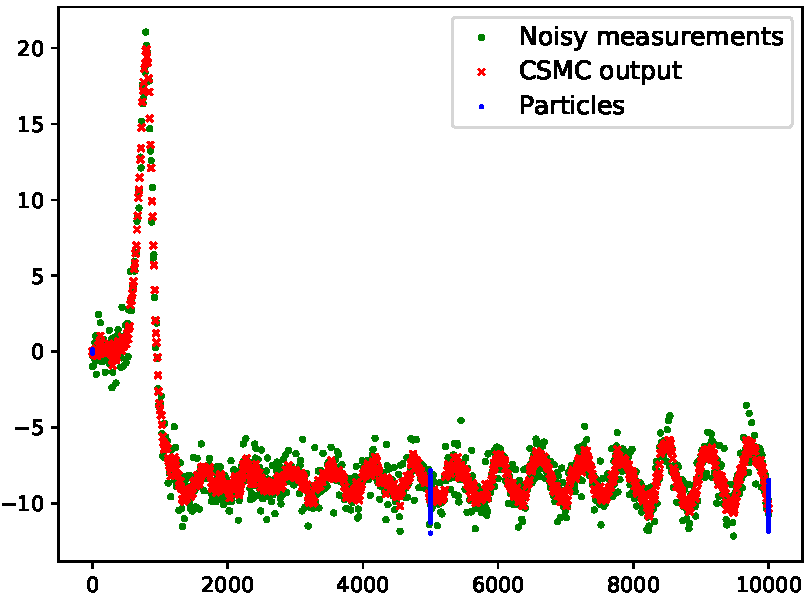
\includegraphics[width=\textwidth]{figures/x-trajectory-data}
        \caption{Trajectory of the $x$ coordinate.} 
        \label{fig:x-trajectory-data}
    \end{subfigure}%
    ~
    \begin{subfigure}{0.49\textwidth}
        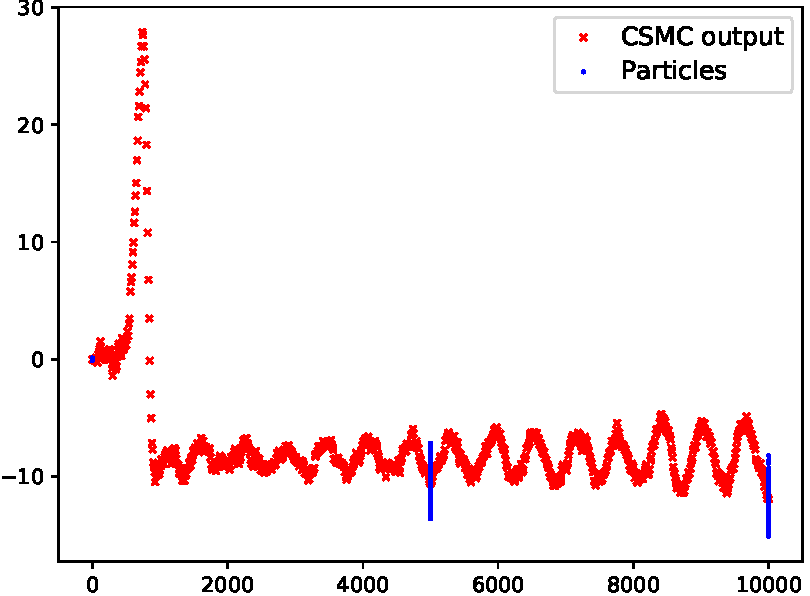
\includegraphics[width=\textwidth]{figures/y-trajectory-data}
        \caption{Trajectory of the $y$ coordinate.} 
        \label{fig:y-trajectory-data}
    \end{subfigure}\\
    \begin{subfigure}{0.49\textwidth}
        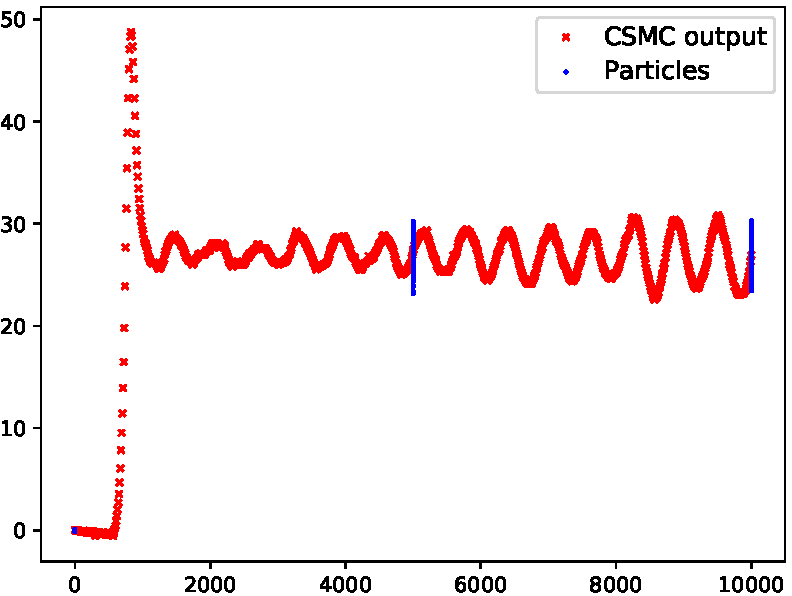
\includegraphics[width=\textwidth]{figures/z-trajectory-data}
        \caption{Trajectory of the $z$ coordinate.} 
        \label{fig:z-trajectory-data}
    \end{subfigure}
    \caption{Estimated trajectories and particles positions at time $t=0, 5, 10$.
    CSMC has been run with 1000 particles.}
\end{figure}

\FloatBarrier

\section{Implementation of an Extended Kalman Filter}

The Extended Kalman Filter amounts to applying a regular Kalman filter to the linearization of the system. Our system can be represented as :


\begin{equation*}
    \begin{cases}
        \vec{x}_{k+1} = F(\vec{x}_k) + \Gamma\vec{u}_k \\
        m_k = x_k + w_k
    \end{cases}.
\end{equation*}

In order to linearize this system, we need to compute the jacobian of $F$, for each time step $k$ :

\begin{equation*}
F_k = 
    \begin{pmatrix}
        1 - a \delta t & a \delta t & 0 \\
        (r - z_k) \delta t & 1 - \delta t & - x_k \delta t \\
        y_k \delta t & x_k \delta t & 1 - b \delta t
    \end{pmatrix}
\end{equation*}

We can then directly apply the Kalman Filter's equations. For prediction :


\[ \vec{\hat{x}}_{k|k-1} = F(\vec{x}_{k-1|k-1}) \]
\[ \vec{P}_{k|k-1} = \vec{F}_{k-1} \vec{P}_{k-1|k-1} \vec{F}_{k-1}^\mathsf{T} + \vec{Q} \]

with $\vec{Q} = \vec{\Gamma} \sigma_u^2$ the covariance matrix of the dynamics' noise.\\
For the update :

\[ \vec{K}_k = \vec{P}_{k|k-1} \vec{H}^\mathsf{T} (\vec{H} ~ \vec{P}_{k|k-1} \vec{H}^\mathsf{T} + R)^{-1} \]

with $R = \sigma_m^2$ and $\vec{H} = 
    \begin{pmatrix}
        1 & 0 & 0 \\
    \end{pmatrix}
$.\\
The updated estimation can then be computed as usual :


\[ \vec{\hat{x}}_{k|k} = \vec{\hat{x}}_{k|k-1} + \vec{K}_k (m_k  - \vec{H} ~ \vec{\hat{x}}_{k|k-1}) \]
\[ \vec{P}_{k|k} = \vec{P}_{k|k-1} - \vec{K}_k ~ \vec{H} ~ \vec{P}_{k|k-1} \]


\end{document}
